\chapter{Results} \label{results}
These are the results obtained from the investigation outlined in \ref{methodology}. Seven volunteers were used in determining the accuracy of the system. They were first measured by the system and then their physical measurements were obtained for comparison. This chapter explores the results obtained for the measurement of the extremities of a human body and the modelling of 3D body parts, together with the observed performance of the user interface respectively.

\section{Length and Extremity Measurement}

This section begins with a presentation of the overall results of the system and a comparison with the aim of the investigation. Subsequent subsections present further performance of specific areas of the system that form the basis of analysis presented in Chapter \ref{analysis}. These sections focus on the following major areas of the system:

\begin{itemize}
	\item The accuracy of measuring key lengths.
	\item The accuracy of each view of measurement (Front, Left, Back and Right) for measuring extremities.
	\item The accuracy of measuring the extremity of each individual limb.
	\item The impact that clothing worn by a person being measured has on the system's accuracy.
	\item Other empirical insights obtained through use and observation of the system. 
\end{itemize}


\subsection{Overall Results}
Below is a summary of the aggregate accuracy of the system and the accuracy per volunteer, together with their personal characteristics. (Table \ref{tab:overallAccuracy})
 
 % Table generated by Excel2LaTeX from sheet 'Overall'
 \begin{table}[htbp]
 	\centering
 	\caption{Overall results of accuracy of system per volunteer}
 	\begin{tabularx}{\textwidth}{|YY|YYY|}
 		\toprule
 		\multicolumn{1}{|Y|}{\textit{\textbf{Volunteer Number}}} & \textit{\textbf{Average Error}} & \multicolumn{1}{Y|}{\textit{\textbf{Build}}} & \multicolumn{1}{Y|}{\textit{\textbf{Height}}} & \textit{\textbf{Clothing}} \\
 		\midrule
 		\multicolumn{1}{|Y|}{\textit{\textbf{1}}} & 28.44\% & \multicolumn{1}{Y|}{Athletic} & \multicolumn{1}{Y|}{Tall} & Loose \\
 		\midrule
 		\multicolumn{1}{|Y|}{\textit{\textbf{2}}} & 17.27\% & \multicolumn{1}{Y|}{Athletic} & \multicolumn{1}{Y|}{Average} & Tight \\
 		\midrule
 		\multicolumn{1}{|Y|}{\textit{\textbf{3}}} & 16.45\% & \multicolumn{1}{Y|}{Athletic} & \multicolumn{1}{Y|}{Tall} & Vest \\
 		\midrule
 		\multicolumn{1}{|Y|}{\textit{\textbf{4}}} & 40.75\% & \multicolumn{1}{Y|}{Slim} & \multicolumn{1}{Y|}{Average} & Loose \\
 		\midrule
 		\multicolumn{1}{|Y|}{\textit{\textbf{5}}} & 20.72\% & \multicolumn{1}{Y|}{Big} & \multicolumn{1}{Y|}{Average} & Loose \\
 		\midrule
 		\multicolumn{1}{|Y|}{\textit{\textbf{6}}} & 19.60\% & \multicolumn{1}{Y|}{Slim} & \multicolumn{1}{Y|}{Short} & Tight \\
 		\midrule
 		\multicolumn{1}{|Y|}{\textit{\textbf{7}}} & 18.83\% & \multicolumn{1}{Y|}{Big} & \multicolumn{1}{Y|}{Average} & Vest \\
 		\midrule
 		\multicolumn{5}{|Y|}{} \\
 		\midrule
 		\multicolumn{2}{|V|}{\textit{\textbf{Total Average Error}}} & \multicolumn{3}{W|}{23.15\%} \\
 		\bottomrule
 	\end{tabularx}%
 	\label{tab:overallAccuracy}%
 \end{table}%
 
As seen in Table \ref{tab:overallAccuracy}, despite the average error of some individual volunteers being outside the desired range of 25\% accuracy, the total average error of the system is 23.15\%. Therefore, the system performed such that it met the requirements of achieving an accuracy better than 25\%, as stipulated in section \ref*{methodologyAim}.

\subsection{Length Performance}
Seen below in Table \ref{tab:lengthResults} are the results of the average accuracy of key lengths obtained after measuring the volunteers in the "Front" view. These lengths are used using joint locations determined by the Kinect's Skeleton Tracking. 
\hl{Insert reference}

% Table generated by Excel2LaTeX from sheet 'Overall'
\begin{table}[htbp]
	\centering
	\caption{Results of the average accuracy of key lengths per volunteer}
	\begin{tabularx}{\textwidth}{|Y|Y|Y|Y|Y|Y|}
		\toprule
		\textit{\textbf{Volunteer Number}} & \textit{\textbf{Left Arm}} & \textit{\textbf{Right Arm}} & \textit{\textbf{Left Leg}} & \textit{\textbf{Right Leg}} & \textit{\textbf{Torso}} \\
		\midrule
		\textit{\textbf{1}} & 6.59\% & 4.35\% & 5.64\% & 3.38\% & 19.52\% \\
		\midrule
		\textit{\textbf{2}} & 11.88\% & 7.66\% & 3.22\% & 10.53\% & 9.55\% \\
		\midrule
		\textit{\textbf{3}} & 12.75\% & 19.49\% & 0.54\% & 0.99\% & 12.15\% \\
		\midrule
		\textit{\textbf{4}} & 8.76\% & 10.64\% & 1.43\% & 0.07\% & 0.51\% \\
		\midrule
		\textit{\textbf{5}} & 2.25\% & 10.17\% & 8.35\% & 7.79\% & 5.64\% \\
		\midrule
		\textit{\textbf{6}} & 4.57\% & 3.08\% & 2.36\% & 3.17\% & 9.38\% \\
		\midrule
		\textit{\textbf{7}} & 2.29\% & 2.54\% & 0.27\% & 2.47\% & 2.98\% \\
		\midrule
		\textit{\textbf{Total Avg Error}} & \textit{\textbf{7.01\%}} & \textit{\textbf{8.27\%}} & \textit{\textbf{3.12\%}} & \textit{\textbf{4.06\%}} & \textit{\textbf{8.53\%}} \\
		\bottomrule
	\end{tabularx}%
	\label{tab:lengthResults}%
\end{table}%

As seen in Table \ref{tab:lengthResults}, all length measurements fell well within the desired accuracy range of 20\%. The most accurate length on average was the "Left Leg" with an accuracy of 3.12\% and the least accurate length on average was the Torso with an accuracy of 8.53\%.

\subsection{View Performance}

Each "view" (Front, Left, Back or Right) of the system has a unique set of characteristics. It is useful to investigate the performance of each of them to better understand their effectiveness in the system as a whole. 

Seen below in Table \ref{tab:viewResults} are the results of the average accuracy of each view obtained after measuring the volunteers in each of the respective views. 

% Table generated by Excel2LaTeX from sheet 'Overall'
\begin{table}[htbp]
	\centering
	\caption{Results of the average accuracy of each view per volunteer}
	\begin{tabularx}{\textwidth}{|Y|Y|Y|Y|Y|}
		\toprule
		\textit{\textbf{Volunteer Number}} & \textit{\textbf{Front}} & \textit{\textbf{Left}} & \textit{\textbf{Back}} & \textit{\textbf{Right}} \\
		\midrule
		\textit{\textbf{1}} & 21.82\% & 29.90\% & 32.61\% & 31.04\% \\
		\midrule
		\textit{\textbf{2}} & 16.58\% & 15.81\% & 20.45\% & 14.60\% \\
		\midrule
		\textit{\textbf{3}} & 17.27\% & 19.01\% & 15.53\% & 13.37\% \\
		\midrule
		\textit{\textbf{4}} & 35.58\% & 58.15\% & 33.58\% & 44.77\% \\
		\midrule
		\textit{\textbf{5}} & 21.06\% & 10.39\% & 24.92\% & 23.47\% \\
		\midrule
		\textit{\textbf{6}} & 11.65\% & 44.58\% & 14.09\% & 17.07\% \\
		\midrule
		\textit{\textbf{7}} & 20.72\% & 19.51\% & 20.60\% & 12.06\% \\
		\midrule
		\textit{\textbf{Total Avg Error}} & \textit{\textbf{20.67\%}} & \textit{\textbf{28.19\%}} & \textit{\textbf{23.11\%}} & \textit{\textbf{22.34\%}} \\
		\bottomrule
	\end{tabularx}%
	\label{tab:viewResults}%
\end{table}%

As seen in Table \ref{tab:viewResults}, the accuracy of the views in descending order are as follows:

\begin{enumerate}
	\item Front
	\item Right
	\item Back
	\item Left
\end{enumerate}

The only view that performed outside the desired accuracy range of 25\% was the "Left" view with an average accuracy of 28.19\%. The Front view performed the best with an accuracy of 20.67\%.  

\subsection{Limb Performance}
Each extremity being measured is subtly different due to various factors such as position, orientation and size. Therefore, understanding how the system performs in these different cases is useful.

Due to the large number of measurements being taken, the results have been split up in terms of upper and lower body measurements.
 
Below is a summary of the aggregate accuracy of the system in measuring upper body limbs per volunteer: (Table \ref{tab:upperBodyResults})

% Table generated by Excel2LaTeX from sheet 'Overall'
\begin{table}[htbp]
	\centering
	\caption{Results of the average accuracy of Upper Body Limbs}
	\begin{tabularx}{\textwidth}{|Y|Y|Y|Y|Y|Y|}
		\toprule
		\textit{\textbf{Volunteer Number}} & \textit{\textbf{Chest}} & \textit{\textbf{Upper Left Arm}} & \textit{\textbf{Lower Left Arm}} & \textit{\textbf{Upper Right Arm}} & \textit{\textbf{Lower Right Arm}} \\
		\midrule
		\textit{\textbf{1}} & 49.50\% & 29.90\% & 10.10\% & 26.35\% & 11.02\% \\
		\midrule
		\textit{\textbf{2}} & 27.84\% & 23.16\% & 9.84\% & 17.74\% & 13.24\% \\
		\midrule
		\textit{\textbf{3}} & 14.58\% & 10.99\% & 24.14\% & 7.33\% & 12.27\% \\
		\midrule
		\textit{\textbf{4}} & 79.55\% & 12.20\% & 26.74\% & 33.79\% & 5.47\% \\
		\midrule
		\textit{\textbf{5}} & 45.85\% & 21.22\% & 8.41\% & 15.16\% & 14.82\% \\
		\midrule
		\textit{\textbf{6}} & 23.39\% & 6.64\% & 15.91\% & 8.46\% & 8.63\% \\
		\midrule
		\textit{\textbf{7}} & 30.70\% & 12.34\% & 12.71\% & 12.02\% & 7.95\% \\
		\midrule
		\textit{\textbf{Total Avg Error}} & \textit{\textbf{38.77\%}} & \textit{\textbf{16.64\%}} & \textit{\textbf{15.41\%}} & \textit{\textbf{17.26\%}} & \textit{\textbf{10.48\%}} \\
		\bottomrule
	\end{tabularx}%
	\label{tab:upperBodyResults}%
\end{table}%

As seen in Table \ref{tab:upperBodyResults}, measurements of the lower and upper portions of both arms fell well within the desired accuracy of 25\%. However, the chest measurements seemed to be significantly more inaccurate with an average of 38.77\%, which is far outside the desired range.

Below is a summary of the aggregate accuracy of the system in measuring lower body limbs per volunteer: (Table \ref{tab:lowerBodyResults})

% Table generated by Excel2LaTeX from sheet 'Overall'
\begin{table}[htbp]
	\centering
	\caption{Results of the average accuracy of Lower Body Limbs}
	\begin{tabularx}{\textwidth}{|Y|Y|Y|Y|Y|Y|}
		\toprule
		\textit{\textbf{Volunteer Number}} & \textit{\textbf{Waist}} & \textit{\textbf{Upper Left Leg}} & \textit{\textbf{Lower Left Leg}} & \textit{\textbf{Upper Right Leg}} & \textit{\textbf{Lower Right Leg}} \\
		\midrule
		\textit{\textbf{1}} & 32.09\% & 31.47\% & 13.58\% & 28.07\% & 44.04\% \\
		\midrule
		\textit{\textbf{2}} & 25.36\% & 15.32\% & 14.18\% & 13.21\% & 6.61\% \\
		\midrule
		\textit{\textbf{3}} & 20.51\% & 13.09\% & 24.62\% & 20.01\% & 10.12\% \\
		\midrule
		\textit{\textbf{4}} & 80.55\% & 13.36\% & 27.94\% & 25.40\% & 48.15\% \\
		\midrule
		\textit{\textbf{5}} & 26.74\% & 16.08\% & 8.56\% & 24.17\% & 15.81\% \\
		\midrule
		\textit{\textbf{6}} & 35.04\% & 20.78\% & 43.78\% & 9.58\% & 17.38\% \\
		\midrule
		\textit{\textbf{7}} & 19.53\% & 23.78\% & 22.77\% & 26.17\% & 16.17\% \\
		\midrule
		\textit{\textbf{Total Avg Error}} & \textit{\textbf{34.26\%}} & \textit{\textbf{19.13\%}} & \textit{\textbf{22.20\%}} & \textit{\textbf{20.95\%}} & \textit{\textbf{22.61\%}} \\
		\bottomrule
	\end{tabularx}%
	\label{tab:lowerBodyResults}%
\end{table}%

As seen in Table \ref{tab:lowerBodyResults}, measurements of the lower and upper portions of both legs fell within the desired accuracy of 25\%. This was similar to the behaviour of the arm measurements, mentioned above. However, they seemed to be slightly more inaccurate with all of the leg measurements having an accuracy tolerance of more than 19\%, whereas the arms all fell within 17.5\%. The waist measurement also followed the behaviour of the chest measurement above, where seemed to be significantly more inaccurate than the leg measurements. It had an average accuracy tolerance of 34.26\%, which is also outside the desired range.

\subsection{Impact of Clothing}

The nature of the system is such that it is sensitive to clothing worn by the measured party. One aim of the system, as stipulated, in section \ref{methodologyAim}, was to make the system more robust to clothing, such that the results are less prone to error.

As such, each of the above measurement results tables have been adjusted to remove the effects of clothing. This has been done by analysing the data set after volunteers with observed "loose" clothing were removed.

Below is the clothing adjusted version of Table \ref{tab:overallAccuracy}. 

% Table generated by Excel2LaTeX from sheet 'Overall'
\begin{table}[htbp]
	\centering
	\caption{Overall results of accuracy of system per volunteer after adjustments for clothing}
	\begin{tabularx}{\textwidth}{|YY|YYY|}
		\toprule
		\multicolumn{1}{|Y|}{\textit{\textbf{Volunteer Number}}} & \textit{\textbf{Average Error}} & \multicolumn{1}{Y|}{\textit{\textbf{Build}}} & \multicolumn{1}{Y|}{\textit{\textbf{Height}}} & \textit{\textbf{Clothing}} \\
		\midrule
		\multicolumn{1}{|Y|}{\textit{\textbf{2}}} & 17.27\% & \multicolumn{1}{Y|}{Athletic} & \multicolumn{1}{Y|}{Average} & Tight \\
		\midrule
		\multicolumn{1}{|Y|}{\textit{\textbf{3}}} & 16.45\% & \multicolumn{1}{Y|}{Athletic} & \multicolumn{1}{Y|}{Tall} & Vest \\
		\midrule
		\multicolumn{1}{|Y|}{\textit{\textbf{6}}} & 19.60\% & \multicolumn{1}{Y|}{Slim} & \multicolumn{1}{c|}{Short} & Tight \\
		\midrule
		\multicolumn{1}{|Y|}{\textit{\textbf{7}}} & 18.83\% & \multicolumn{1}{Y|}{Big} & \multicolumn{1}{c|}{Average} & Vest \\
		\midrule
		\multicolumn{5}{|Y|}{} \\
		\midrule
		\multicolumn{2}{|V|}{\textit{\textbf{Total Error Average}}} & \multicolumn{3}{W|}{\textit{\textbf{18.04\%}}} \\
		\bottomrule
	\end{tabularx}%
	\label{tab:overallResultsClothingAdj}%
\end{table}%

It is clear from Table \ref{tab:overallResultsClothingAdj} that the system performs significantly better when loose clothing is not worn by the volunteer. The new overall average accuracy of the system improved to 18.04\%, which is well within the desired range of 25\%. This improvement, from 23.15\%, due to the removal of 3 Volunteers with loose clothing means the average accuracy of these Volunteers is 29.96\%. Therefore, clothing worsened the overall accuracy of an individuals reading by approximately 66.08\%. This falls outside the desired range of 30\%. 

The same behaviour can be observed for the accuracy of the views and the different limbs.

In the adjusted version of Table \ref{tab:viewResults} (Table \ref{tab:viewResultsClothingAdj}), the performance of all the views improve. Additionally, the "Left" view now also falls within the desired 25\% range and all the other views fall within 18\%. 

% Table generated by Excel2LaTeX from sheet 'Overall'
\begin{table}[htbp]
	\centering
	\caption{Results of the average accuracy of each view per volunteer after adjustments for clothing}
	\begin{tabularx}{\textwidth}{|Y|Y|Y|Y|Y|}
		\toprule
		\textit{\textbf{Volunteer Number}} & \textit{\textbf{Front}} & \textit{\textbf{Left}} & \textit{\textbf{Back}} & \textit{\textbf{Right}} \\
		\midrule
		\textit{\textbf{2}} & 16.58\% & 15.81\% & 20.45\% & 14.60\% \\
		\midrule
		\textit{\textbf{3}} & 17.27\% & 19.01\% & 15.53\% & 13.37\% \\
		\midrule
		\textit{\textbf{6}} & 11.65\% & 44.58\% & 14.09\% & 17.07\% \\
		\midrule
		\textit{\textbf{7}} & 20.72\% & 19.51\% & 20.60\% & 12.06\% \\
		\midrule
		\textit{\textbf{Total Avg Error}} & \textit{\textbf{16.55\%}} & \textit{\textbf{24.73\%}} & \textit{\textbf{17.67\%}} & \textit{\textbf{14.27\%}} \\
		\bottomrule
	\end{tabularx}%
	\label{tab:viewResultsClothingAdj}%
\end{table}%

As for the adjusted upper and lower body measurements (Table \ref{tab:upperBodyResultsClothingAdj} and Table  \ref{tab:lowerBodyResultsClothingAdj} respectively), all of the measurements, except for the "Lower Left Leg" measurement (increased to 26.34\% which is outside the desired range) either improved in accuracy or remained within 1\% of its previous accuracy. The "Chest" measurement is now within the desired accuracy range of 25\% with a value of 24.13\%. The "Waist" measurement also greatly improved, however, is still narrowly outside the desired range with an accuracy of 25.11\%   

% Table generated by Excel2LaTeX from sheet 'Overall'
\begin{table}[htbp]
	\centering
	\caption{Results of the average accuracy of Upper Body Limbs after adjustments for clothing}
	\begin{tabularx}{\textwidth}{|Y|Y|Y|Y|Y|Y|}
		\toprule
		\textit{\textbf{Volunteer Number}} & \textit{\textbf{Chest}} & \textit{\textbf{Upper Left Arm}} & \textit{\textbf{Lower Left Arm}} & \textit{\textbf{Upper Right Arm}} & \textit{\textbf{Lower Right Arm}} \\
		\midrule
		\textit{\textbf{2}} & 27.84\% & 23.16\% & 9.84\% & 17.74\% & 13.24\% \\
		\midrule
		\textit{\textbf{3}} & 14.58\% & 10.99\% & 24.14\% & 7.33\% & 12.27\% \\
		\midrule
		\textit{\textbf{6}} & 23.39\% & 6.64\% & 15.91\% & 8.46\% & 8.63\% \\
		\midrule
		\textit{\textbf{7}} & 30.70\% & 12.34\% & 12.71\% & 12.02\% & 7.95\% \\
		\midrule
		\textit{\textbf{Total Avg Error}} & \textit{\textbf{24.13\%}} & \textit{\textbf{13.28\%}} & \textit{\textbf{15.65\%}} & \textit{\textbf{11.39\%}} & \textit{\textbf{10.52\%}} \\
		\bottomrule
	\end{tabularx}%
	\label{tab:upperBodyResultsClothingAdj}%
\end{table}%

% Table generated by Excel2LaTeX from sheet 'Overall'
\begin{table}[htbp]
	\centering
	\caption{Results of the average accuracy of Lower Body Limbs after adjustments for clothing}
	\begin{tabularx}{\textwidth}{|Y|Y|Y|Y|Y|Y|}
		\toprule
		\textit{\textbf{Volunteer Number}} & \textit{\textbf{Waist}} & \textit{\textbf{Upper Left Leg}} & \textit{\textbf{Lower Left Leg}} & \textit{\textbf{Upper Right Leg}} & \textit{\textbf{Lower Right Leg}} \\
		\midrule
		\textit{\textbf{2}} & 25.36\% & 15.32\% & 14.18\% & 13.21\% & 6.61\% \\
		\midrule
		\textit{\textbf{3}} & 20.51\% & 13.09\% & 24.62\% & 20.01\% & 10.12\% \\
		\midrule
		\textit{\textbf{6}} & 35.04\% & 20.78\% & 43.78\% & 9.58\% & 17.38\% \\
		\midrule
		\textit{\textbf{7}} & 19.53\% & 23.78\% & 22.77\% & 26.17\% & 16.17\% \\
		\midrule
		\textit{\textbf{Total Avg Error}} & \textit{\textbf{25.11\%}} & \textit{\textbf{18.24\%}} & \textit{\textbf{26.34\%}} & \textit{\textbf{17.24\%}} & \textit{\textbf{12.57\%}} \\
		\bottomrule
	\end{tabularx}%
	\label{tab:lowerBodyResultsClothingAdj}%
\end{table}%

\subsection{Uncertainty}
The uncertainty of each limb measurement in each view can be seen in Table \ref{tab:upperBodyUncertainty} and Table \ref{tab:lowerBodyUncertainty}. As mentioned in \hl{(Insert Reference)}, these were calculated assuming a Gaussian distribution of measured values.\\ 
\textit{Note: The values of \#N/A represent values that are not available in the respective view - I.e. The left hand side of the body cannot be seen when the volunteer is orientated right and as such are not available for measurement in that view}

\begin{figure}[ht]
	\centering
	{%
		\setlength{\fboxsep}{0pt}%
		\setlength{\fboxrule}{0.5pt}%
		\fbox{
			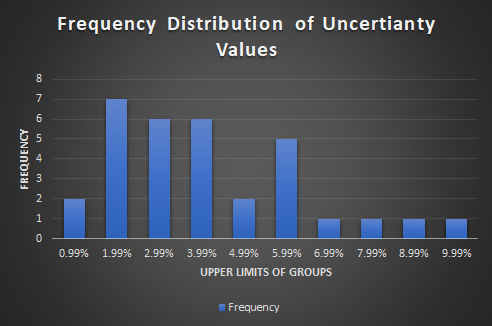
\includegraphics[width=0.7\textwidth]{FreqDistUncertainties.png}
	}}
	\caption{A histogram depicting the frequency distribution of the uncertainty values displayed in Table \ref{tab:upperBodyUncertainty} and Table \ref{tab:lowerBodyUncertainty}}
	\label{fig:uncertaintyFreqDist}
\end{figure}

As seen in Figure \ref{fig:uncertaintyFreqDist} below, all the uncertainty values calculated for each limb in the different views fell within the desired range of $<10\%$. Additionally, majority of the values actually fell within the range of 0-6\%. 

% Table generated by Excel2LaTeX from sheet 'Overall'
\begin{table}[htbp]
	\centering
	\caption{Results of the average uncertainty $(U_n)$ of Upper Body Limbs per view}
	\begin{tabularx}{\textwidth}{|Y|Y|Y|Y|Y|Y|}
		\toprule
		\textit{\textbf{View}} & \textit{\textbf{Chest}} & \textit{\textbf{Upper Left Arm}} & \textit{\textbf{Lower Left Arm}} & \textit{\textbf{Upper Right Arm}} & \textit{\textbf{Lower Right Arm}} \\
		\midrule
		\textit{\textbf{Front}} & 1.19\% & 3.84\% & 9.37\% & 3.48\% & 5.28\% \\
		\midrule
		\textit{\textbf{Left}} & 2.03\% & 3.50\% & 6.82\% & \#N/A & \#N/A \\
		\midrule
		\textit{\textbf{Back}} & 1.64\% & 3.29\% & 5.41\% & 3.02\% & 4.47\% \\
		\midrule
		\textit{\textbf{Right}} & 0.91\% & \#N/A & \#N/A & 5.00\% & 5.74\% \\
		\midrule
		\textit{\textbf{Total Avg $(U_n)$}} & \textit{\textbf{1.44\%}} & \textit{\textbf{3.54\%}} & \textit{\textbf{7.20\%}} & \textit{\textbf{3.83\%}} & \textit{\textbf{5.16\%}} \\
		\bottomrule
	\end{tabularx}%
	\label{tab:upperBodyUncertainty}%
\end{table}%

% Table generated by Excel2LaTeX from sheet 'Overall'
\begin{table}[htbp]
	\centering
	\caption{Results of the average uncertainty $(U_n)$ of Lower Body Limbs per view}
	\begin{tabularx}{\textwidth}{|Y|Y|Y|Y|Y|Y|}
		\toprule
		\textit{\textbf{View}} & \textit{\textbf{Waist}} & \textit{\textbf{Upper Left Leg}} & \textit{\textbf{Lower Left Leg}} & \textit{\textbf{Upper Right Leg}} & \textit{\textbf{Lower Right Leg}} \\
		\midrule
		\textit{\textbf{Front}} & 1.25\% & 1.26\% & 2.86\% & 3.41\% & 5.72\% \\
		\midrule
		\textit{\textbf{Left}} & 2.36\% & 1.34\% & 8.01\% & \#N/A & \#N/A \\
		\midrule
		\textit{\textbf{Back}} & 0.91\% & 2.42\% & 2.70\% & 1.16\% & 1.08\% \\
		\midrule
		\textit{\textbf{Right}} & 2.03\% & \#N/A & \#N/A & 4.62\% & 7.79\% \\
		\midrule
		\textit{\textbf{Total Avg $(U_n)$}} & \textit{\textbf{1.64\%}} & \textit{\textbf{1.67\%}} & \textit{\textbf{4.52\%}} & \textit{\textbf{3.06\%}} & \textit{\textbf{4.86\%}} \\
		\bottomrule
	\end{tabularx}%
	\label{tab:lowerBodyUncertainty}%
\end{table}%

Upon closer inspection of Table \ref{tab:upperBodyUncertainty} and Table \ref{tab:lowerBodyUncertainty}, it is clear that all the individual and average uncertainty values fell within the desired range of 10\%. The most reliable reading (One with the smallest uncertainty) was the "Chest" measurement with a 1.44\% uncertainty. As a group, the leg measurements seemed to be more reliable than the arm measurements as all of the average leg uncertainties fell within 5\%. On the other end of the spectrum, the measurement with the greatest average uncertainty was the "Left Arm" with an uncertainty of 7.20\%.

\subsection{Other Empirical Observations} \label{empiricalObservations}

Apart from the above presented tables of results, other observations were made of the system during its use. These observations are explained in each of the following subsections:

\subsubsection{Background Removal Error} \label{backgroundRemovalError}
There were instances where the Background Removal functionality of the Kinect performed with error. These errors presented themselves in two manners:

\begin{figure}[ht]
	\centering
	{%
		\setlength{\fboxsep}{0pt}%
		\setlength{\fboxrule}{0.5pt}%
		\fbox{
	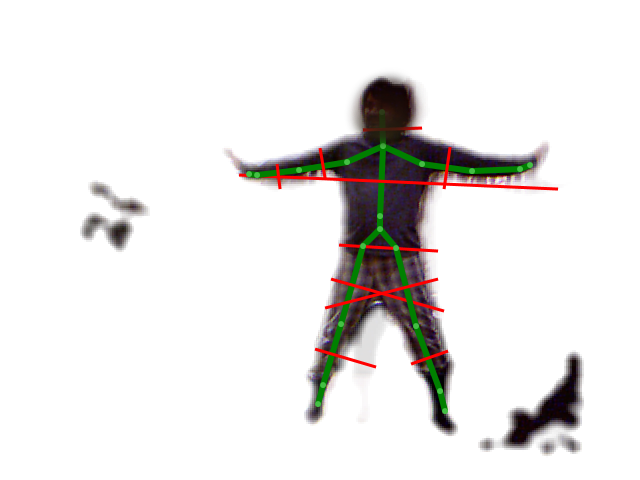
\includegraphics[width=0.7\textwidth]{ErrorExample_Blurred.png}
	}}
	\caption{An example of failures of extremity measurements due to background removal and padding errors detected in early testing}
	\label{fig:errorExample}
\end{figure}

\begin{figure}[ht]
	\centering
	{%
		\setlength{\fboxsep}{0pt}%
		\setlength{\fboxrule}{0.5pt}%
		\fbox{
	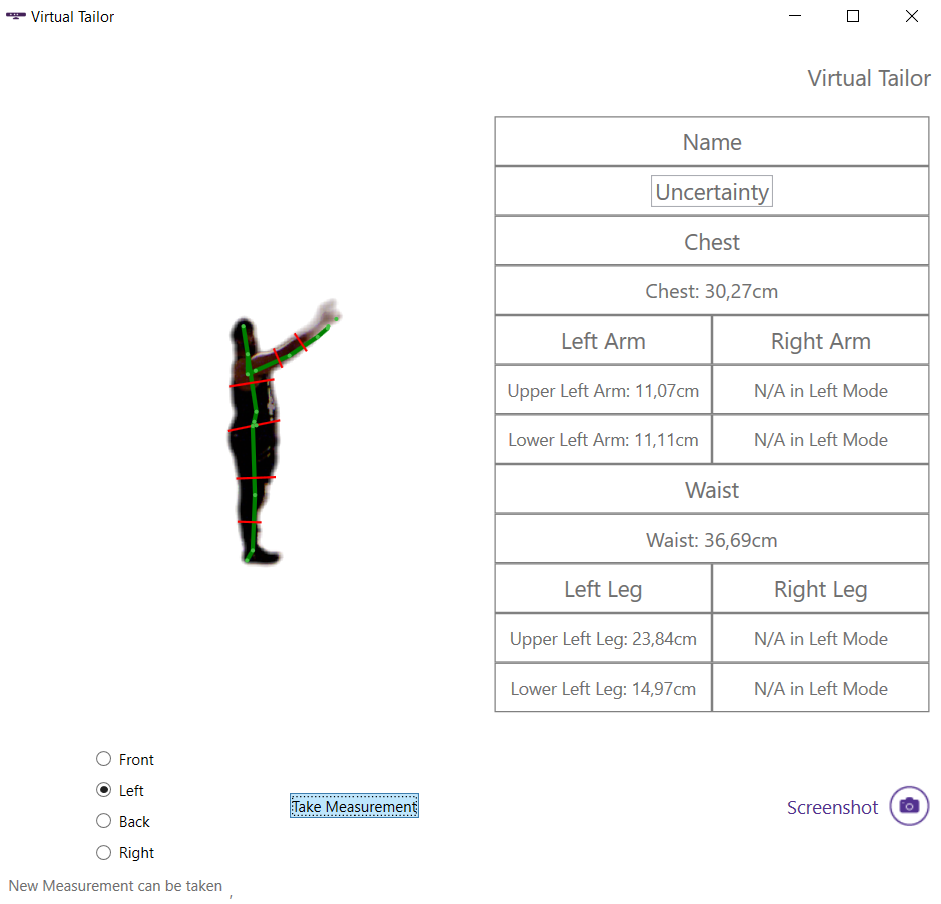
\includegraphics[width=0.7\textwidth]{Uncertainty_Left4.png}
	}}
	\caption{An example of trailing pixels detected by background removal that forms part of padding errors}
	\label{fig:uncertaintyLeft4}
\end{figure}

\begin{figure}[ht]
	\centering
	{%
		\setlength{\fboxsep}{0pt}%
		\setlength{\fboxrule}{0.5pt}%
		\fbox{
	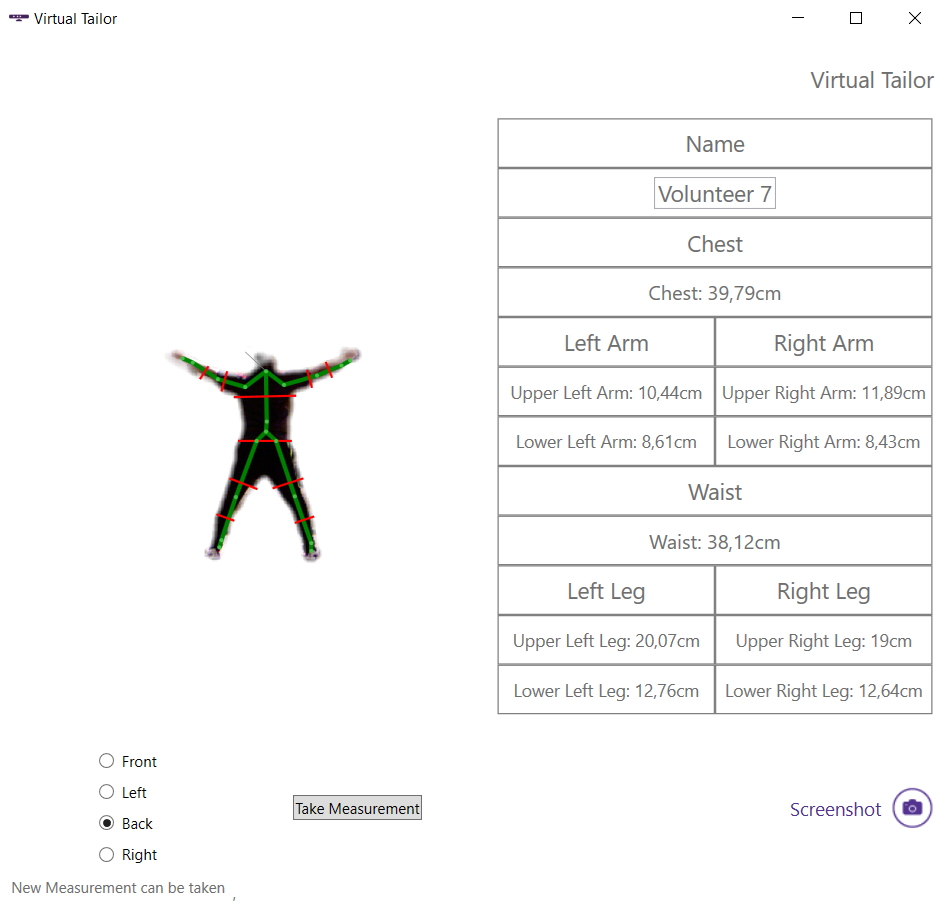
\includegraphics[width=0.7\textwidth]{Volunteer7_Back.png}
	}}
	\caption{An example of the presence of a background removal error relating to incorrect pixel removal during final testing}
	\label{fig:volunteer7Back}
\end{figure}

\begin{figure}[ht]
	\centering
	{%
		\setlength{\fboxsep}{0pt}%
		\setlength{\fboxrule}{0.5pt}%
		\fbox{
			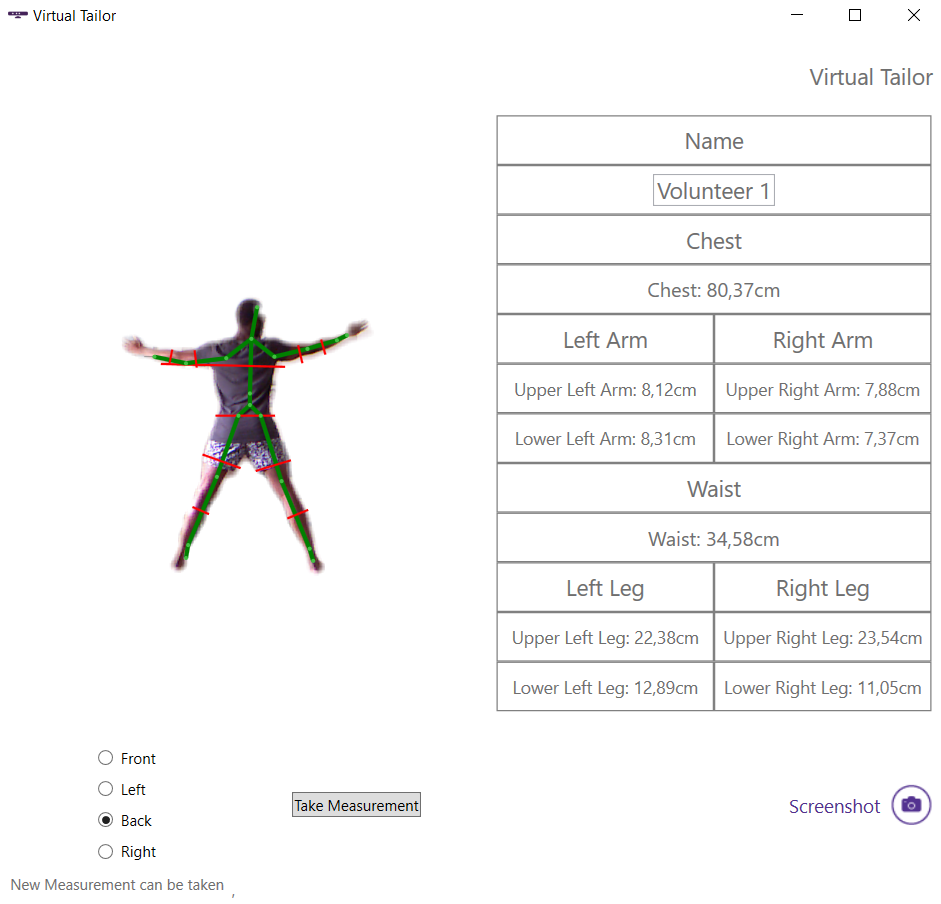
\includegraphics[width=0.7\textwidth]{Volunteer1_Back.png}
	}}
	\caption{An example of failures of extremity measurements due to background removal and padding errors during final testing}
	\label{fig:volunteer1Back}
\end{figure}

\paragraph{Extra Padding}
During early and final testing of the system, it was observed that the output background removed picture had extra padding around the detected human in some instances. This extra padding consisted of background pixels that should have been removed. 

An example of an early test with the above error can be seen in Figure \ref{fig:errorExample}. In this image, it can be clearly seen that extra background pixels have been included in regions under the outstretched arms, on the sides of the torso and underneath the groin. 

An additional caveat to the above error was also detected. It was observed that when the detected human was processed while moving, trailing pixels from the previous position would be included in the image and form part of the padding.

This was present in both early testing and final testing. In Figure \ref{fig:errorExample}, mentioned above, this can be clearly seen as the left leg has a "ghost" or "trailing" leg present. An example of a final test with trailing pixels can be seen in Figure \ref{fig:uncertaintyLeft4}. In this image, careful inspection of the extended hand reveals that trailing pixels are present due to movement of the detected human.

\paragraph{Incorrect Pixel Removal}
The other error present as a result of the Background Removal functionality is the incorrect pixel removal of pixels that form part of the detected human. The parts of the body that suffered the most frequently from this error are the parts at the extremes (E.g. Head, hands, "feet, etc.). Additionally, the view in which incorrect pixel removal from the "Head" was the most prevalent, was the "Back" view. 

An example of a final test with incorrect pixel removal can be seen in Figure \ref{fig:volunteer7Back}. Careful inspection of this image reveals that pixels that form part of the head and hands of the detected human have been incorrectly removed. 

\subsubsection{Overlap Error}
It was observed that occasionally, the system failed to detect a correct extremity. As mentioned in \hl{Insert Reference}, measuring extremities assumes that an outline of a limb will be against a background and thus, after the background is removed, will be clearly distinguishable. However, it was observed that in instances where an outline overlapped with another part of the body or the extra background padding mentioned in section \ref{backgroundRemovalError} above, the outline would not be detected by the system. 

A clear example can be seen in Figure \ref{fig:errorExample}. The "Chest", "Upper Right Leg", "Upper Left Leg" and "Lower Left Leg" in this image have been erroneously extended due to overlap errors. The "Upper Leg" measurements were extended due to overlap of the detected human's thighs, thus making their division indistinguishable. The "Chest" and the "Lower Left Leg measurement were both extended due to overlap caused by background padding. Respectively, they were caused by the padding underneath the arms and trailing pixels of the left leg. 

Examples of this error during final testing can be seen in Figure \ref{fig:volunteer1Back} and Figure \ref{fig:volunteer1Right}. In Figure \ref{fig:volunteer1Back}, the overlap error is present in the "Chest" measurement as its plane of measurement intersected with the right arm, which was too low in this case. In Figure \ref{fig:volunteer1Right}, the overlap error is present in the "Lower Right Leg" as its plane of measurement intersected with the "Lower Left Leg". The volunteer in this case was facing right for a "Right" view measurement. However, the volunteer's legs were not together and slightly ajar, thus creating an unwanted overlap.

\begin{figure}[ht]
	\centering
	{%
		\setlength{\fboxsep}{0pt}%
		\setlength{\fboxrule}{0.5pt}%
		\fbox{
			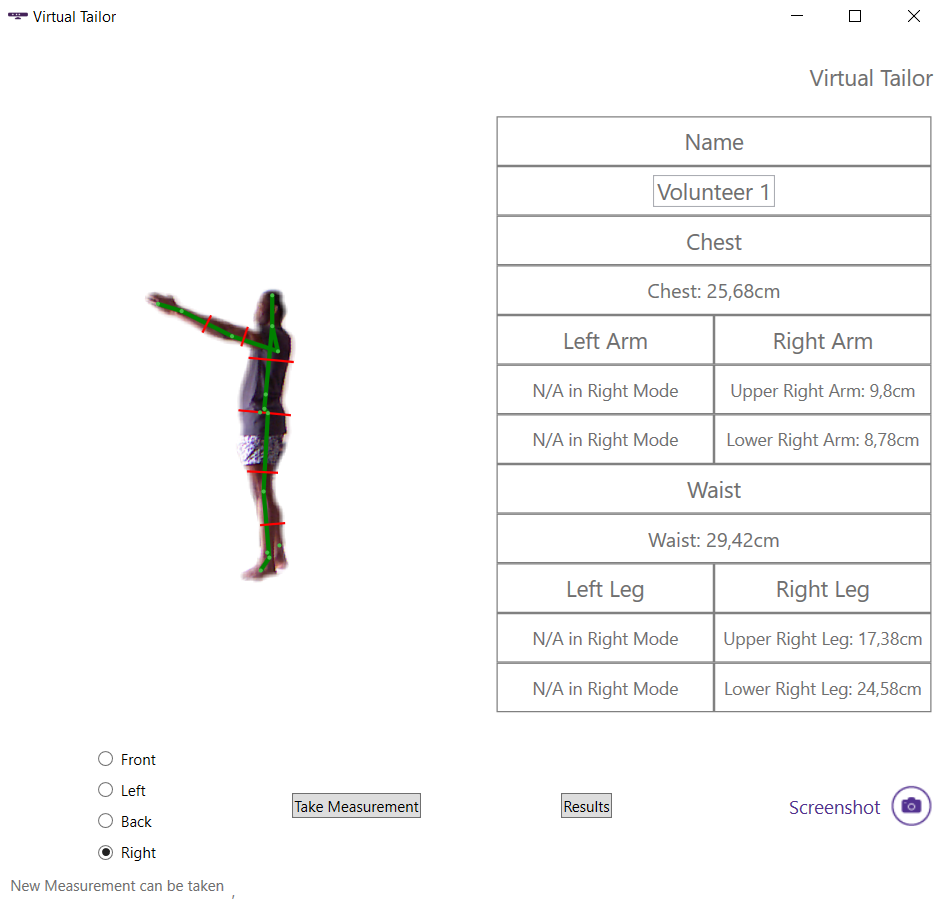
\includegraphics[width=0.7\textwidth]{Volunteer1_Right.png}
	}}
	\caption{An example of overlap error due to orientation during final testing}
	\label{fig:volunteer1Right}
\end{figure}

\subsubsection{Missing Measurements}
During final testing, it was observed that occasionally, certain limb measurements were not processed properly and as a result, were not available. This manifested in certain limb measurements returning a value of "0cm", in its corresponding location on the user interface, when a non-zero value was expected. 

This error was observed in four individual limb readings belonging to two separate volunteers. The corresponding volunteer, view, limb details of the missing measurement are listed below, together with the figure in which it can be seen:

\begin{enumerate}
	\item Volunteer 3 - Back View - Upper Right Arm - Figure \ref{fig:volunteer3Back}
	\item Volunteer 3 - Right View - Upper Right Arm - Figure \ref{fig:volunteer3Right}
	\item Volunteer 4 - Back View - Lower Right Arm - Figure \ref{fig:volunteer4Back}
	\item Volunteer 4 - Left View - Lower Left Arm - Figure \ref{fig:volunteer4Left}
\end{enumerate}	  

\begin{figure}[ht]
	\centering
	{%
		\setlength{\fboxsep}{0pt}%
		\setlength{\fboxrule}{0.5pt}%
		\fbox{
			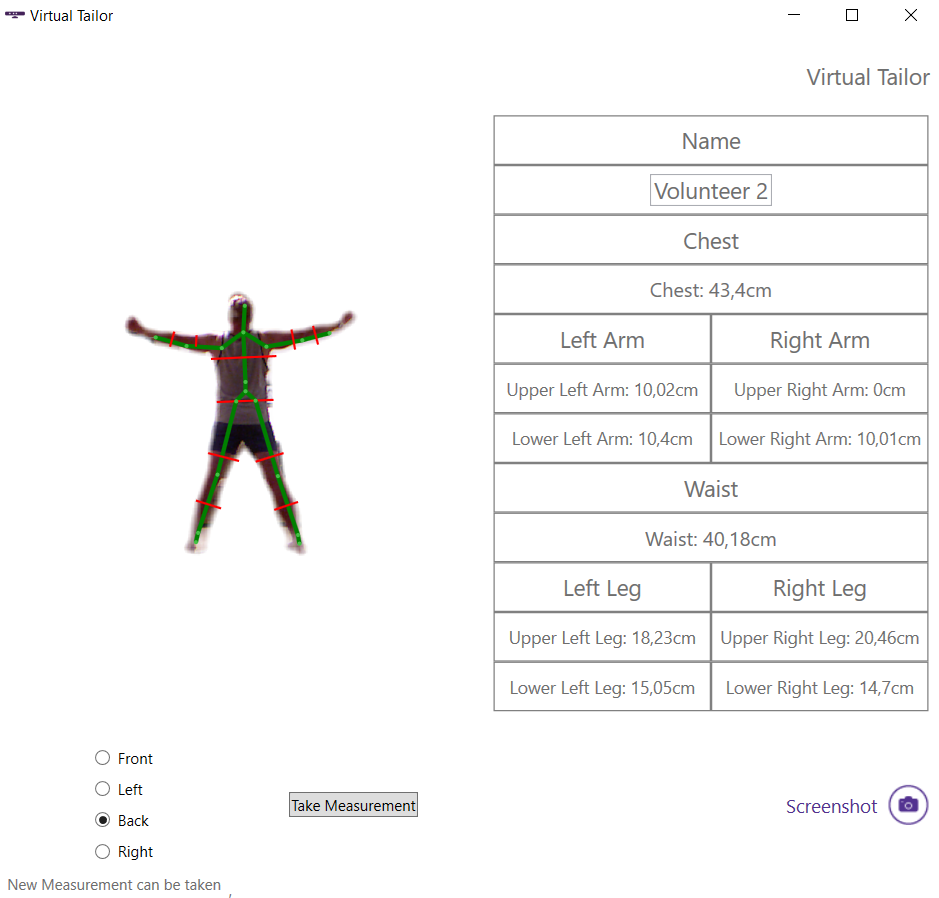
\includegraphics[width=0.7\textwidth]{Volunteer3_Back.png}
	}}
	\caption{An example of a missing measurement - Volunteer 3 - Back View - Upper Right Arm}
	\label{fig:volunteer3Back}
\end{figure}

\begin{figure}[ht]
	\centering
	{%
		\setlength{\fboxsep}{0pt}%
		\setlength{\fboxrule}{0.5pt}%
		\fbox{
			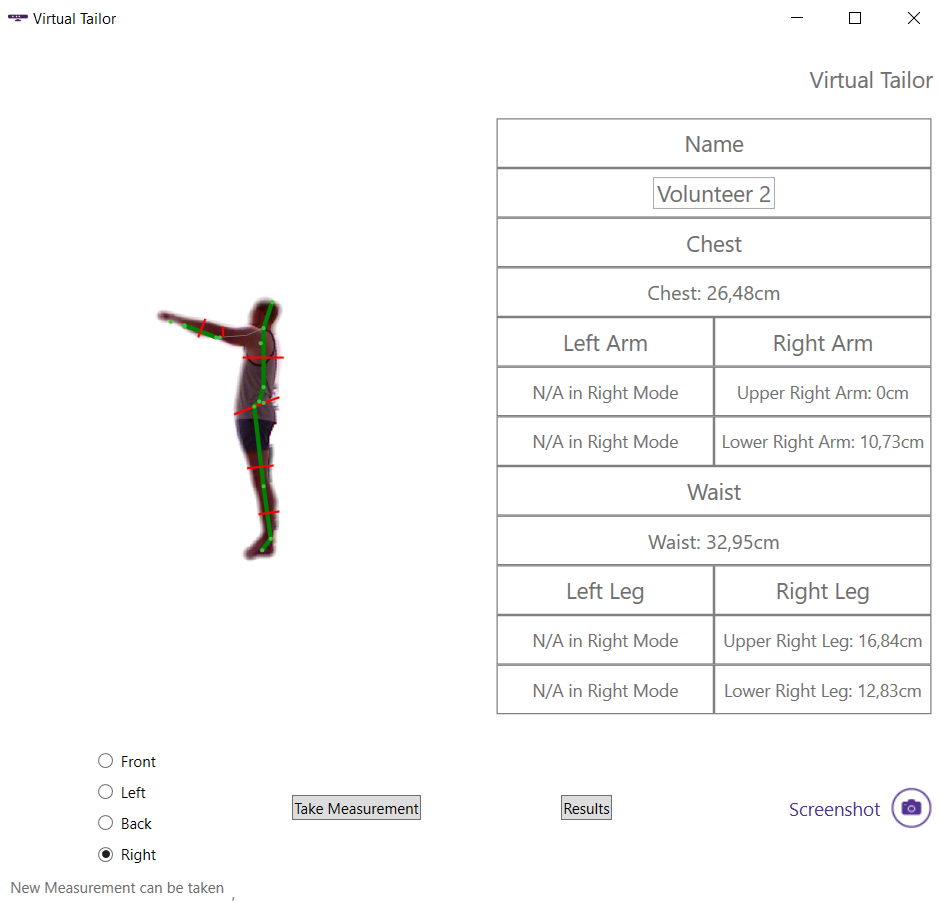
\includegraphics[width=0.7\textwidth]{Volunteer3_Right.png}
	}}
	\caption{An example of a missing measurement - Volunteer 3 - Right View - Upper Right Arm}
	\label{fig:volunteer3Right}
\end{figure}

\begin{figure}[ht]
	\centering
	{%
		\setlength{\fboxsep}{0pt}%
		\setlength{\fboxrule}{0.5pt}%
		\fbox{
			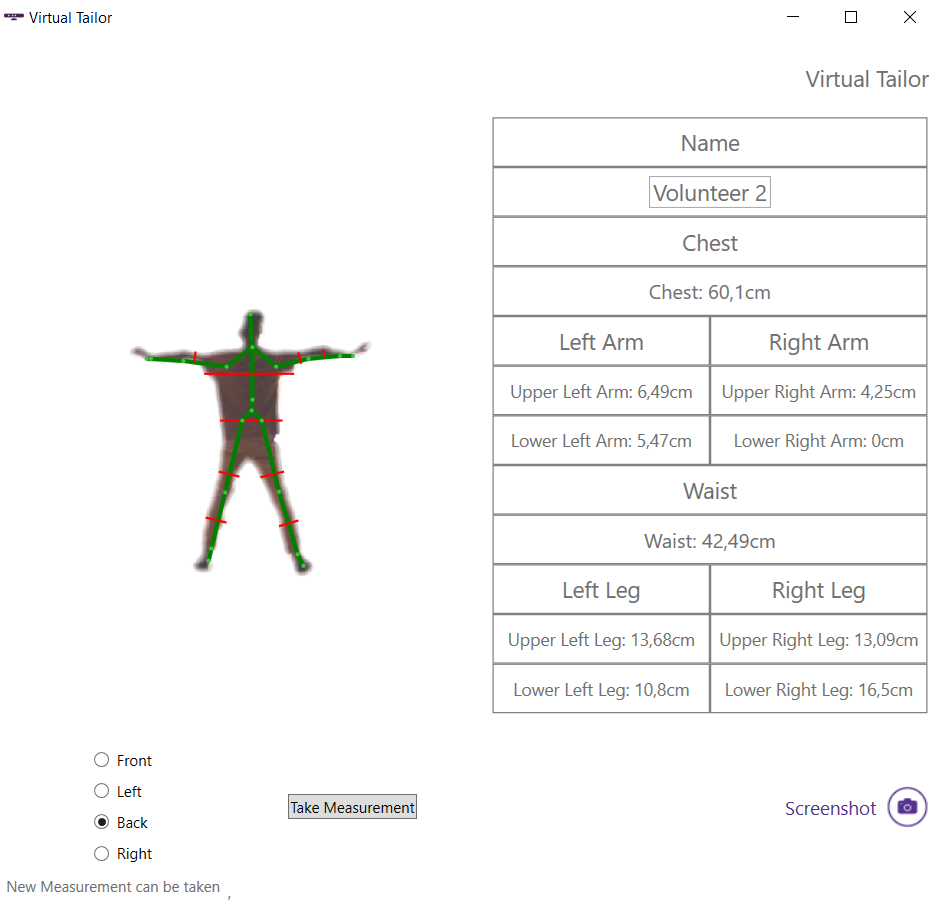
\includegraphics[width=0.7\textwidth]{Volunteer4_Back.png}
	}}
	\caption{An example of a missing measurement - Volunteer 4 - Back View - Lower Right Arm}
	\label{fig:volunteer4Back}
\end{figure}

\begin{figure}[ht]
	\centering
	{%
		\setlength{\fboxsep}{0pt}%
		\setlength{\fboxrule}{0.5pt}%
		\fbox{
			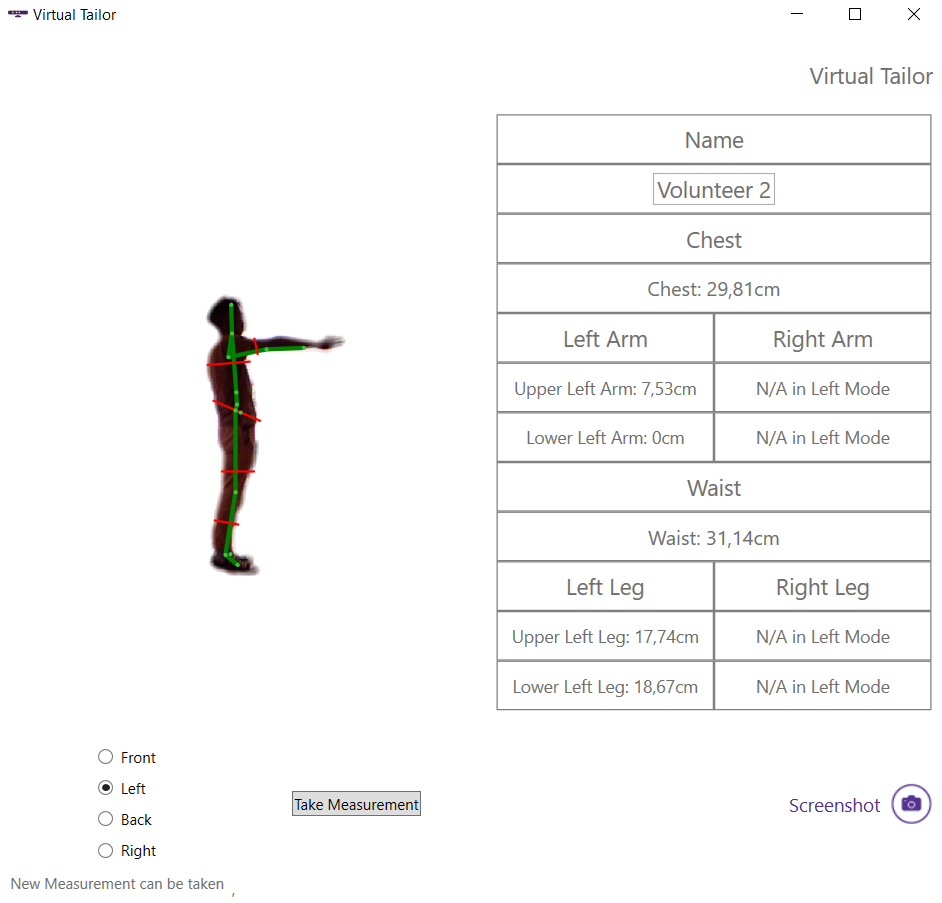
\includegraphics[width=0.7\textwidth]{Volunteer4_Left.png}
	}}
	\caption{An example of a missing measurement - Volunteer 3 - Back View - Lower Left Arm}
	\label{fig:volunteer4Left}
\end{figure}

\subsubsection{Incorrect Waist Plane}
The last error that was observed during final testing was the occurrence of an incorrect waist plane when taking a measurement from either the "Left" or "Right" view. 

In Figure \ref{fig:waistPlaneError}, the "Front" view of the volunteer is shown on the left side of the image and the "Right" view on the right side. It is evident that the waist plane in the "Front" view is correct as it is drawn across the hips in an almost horizontal fashion. The waist plane in all views should follow this pattern. However, the waist plane in the "Right" view is severely angled and deviates from the horizontal. As such, the measurement obtained would be incorrect and often inflated. 

Additionally, the deviation from the horizontal (Or the angle fo the waist plane) varied depending on the rotation of the volunteers body, thus producing unpredictable results. An example of this changing deviation can be seen in Figure \ref{fig:volunteer2Left}. Here, the "Left" view measurement of the same volunteer that appears in Figure \ref{fig:waistPlaneError} is shown. However, it is evident that the deviation of the waist plane in the "Left" and "Right" views is not consistent. 

\begin{figure}[ht]
	\centering
	{%
		\setlength{\fboxsep}{0pt}%
		\setlength{\fboxrule}{0.5pt}%
		\fbox{
			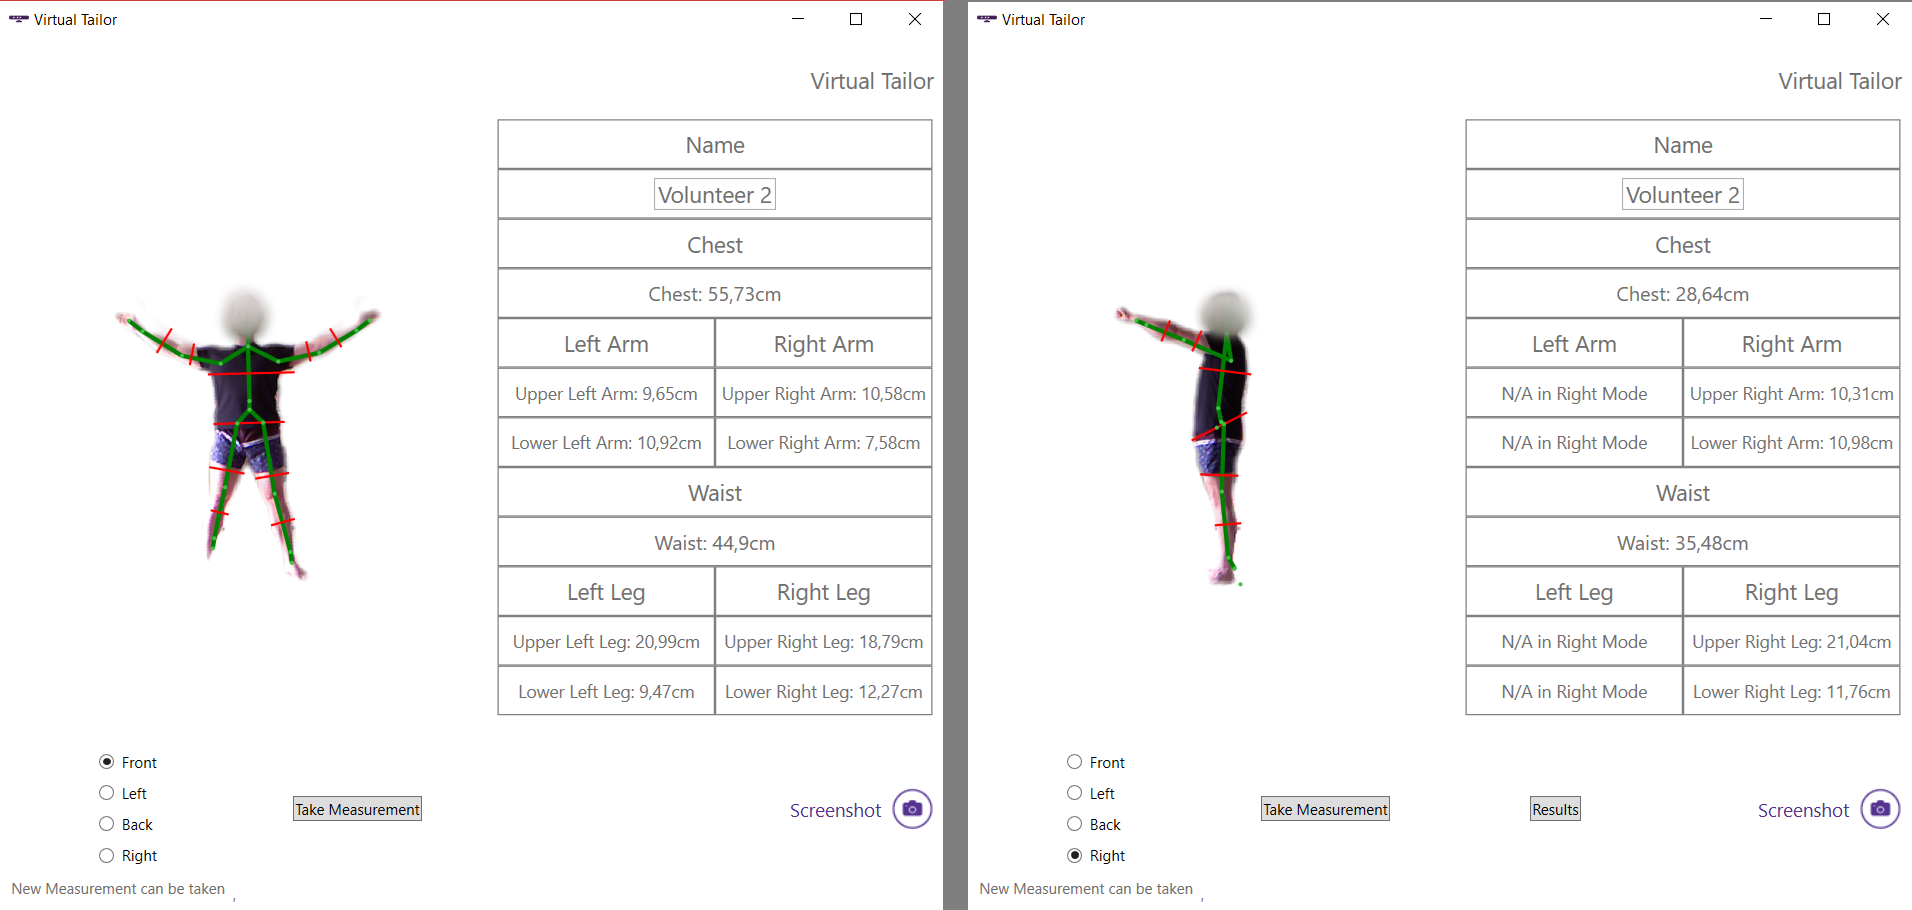
\includegraphics[width=0.7\textwidth]{WaistPlaneError.png}
	}}
	\caption{A comparison of the "Front" and "Right" view measurements volunteer 2 to illustrate the waist plane error}
	\label{fig:waistPlaneError}
\end{figure}

\begin{figure}[ht]
	\centering
	{%
		\setlength{\fboxsep}{0pt}%
		\setlength{\fboxrule}{0.5pt}%
		\fbox{
			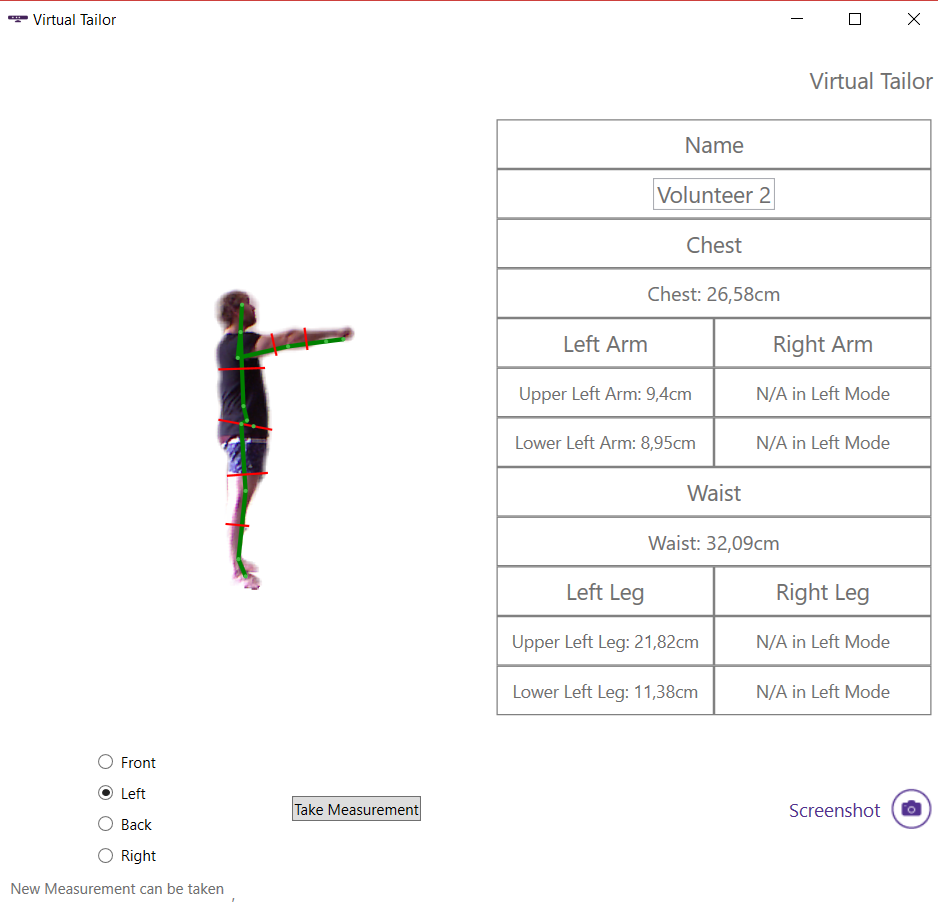
\includegraphics[width=0.7\textwidth]{Volunteer2_Left.png}
	}}
	\caption{A comparison of the "Front" and "Right" view measurements volunteer 2 to illustrate the waist plane error}
	\label{fig:volunteer2Left}
\end{figure}

\section{3D Modelling}
This section details the results of the accuracy of the two models used for calculating the 3D circumference. 

\subsection{Ellipse Model}
Table \ref{tab:ovalUpper} and Table \ref{tab:ovalLower} are summaries of the average accuracy of using the ellipse model to the various upper and lower body limbs.

Volunteers 1, 2, 3 and 4 were used to test the ellipse model. However, the results of Volunteer 1 were erroneous due to a mistake made during recording of the results. (This mistake is dealt with in Section \ref{UIObservations})

% Table generated by Excel2LaTeX from sheet '3D Modelling'
\begin{table}[htbp]
	\centering
	\caption{Results of circumference modelling of upper body limbs using the ellipse model}
	\begin{tabularx}{\textwidth}{|Y|Y|Y|Y|Y|Y|}
		\toprule
		\textit{\textbf{Volunteer Number}} & \textit{\textbf{Chest}} & \textit{\textbf{Upper Left Arm}} & \textit{\textbf{Lower Left Arm}} & \textit{\textbf{Upper Right Arm}} & \textit{\textbf{Lower Right Arm}} \\
		\midrule
		\textit{\textbf{2}} & 129.87\% & 54.58\% & 104.72\% & 69.27\% & 97.32\% \\
		\midrule
		\textit{\textbf{3}} & 101.21\% & 111.53\% & 48.71\% & \#N/A & 105.13\% \\
		\midrule
		\textit{\textbf{4}} & 199.89\% & 103.06\% & \#N/A & 50.86\% & 59.77\% \\
		\midrule
		\textit{\textbf{Total Avg Error}} & \textit{\textbf{143.66\%}} & \textit{\textbf{89.72\%}} & \textit{\textbf{76.72\%}} & \textit{\textbf{60.06\%}} & \textit{\textbf{87.41\%}} \\
		\bottomrule
	\end{tabularx}%
	\label{tab:ovalUpper}%
\end{table}%

% Table generated by Excel2LaTeX from sheet '3D Modelling'
\begin{table}[htbp]
	\centering
	\caption{Results of circumference modelling of lower body limbs using the ellipse model}
	\begin{tabularx}{\textwidth}{|Y|Y|Y|Y|Y|Y|}
		\toprule
		\textit{\textbf{Volunteer Number}} & \textit{\textbf{Waist}} & \textit{\textbf{Upper Left Leg}} & \textit{\textbf{Lower Left Leg}} & \textit{\textbf{Upper Right Leg}} & \textit{\textbf{Lower Right Leg}} \\
		\midrule
		\textit{\textbf{2}} & 135.79\% & 117.74\% & 72.41\% & 107.70\% & 75.23\% \\
		\midrule
		\textit{\textbf{3}} & 119.85\% & 103.90\% & 110.44\% & 80.61\% & 95.57\% \\
		\midrule
		\textit{\textbf{4}} & 190.44\% & 113.02\% & 171.66\% & 180.64\% & 156.81\% \\
		\midrule
		\textit{\textbf{Total Avg Error}} & \textit{\textbf{148.70\%}} & \textit{\textbf{111.55\%}} & \textit{\textbf{118.17\%}} & \textit{\textbf{122.98\%}} & \textit{\textbf{109.20\%}} \\
		\bottomrule
	\end{tabularx}%
	\label{tab:ovalLower}%
\end{table}%

As seen in Table \ref{tab:ovalUpper} and Table \ref{tab:ovalLower}, the ellipse model was not successful in approximating the 3D circumference of the various limbs. All of the average accuracies calculated were above 60\% and the worst performing measurement being the "Waist" with an average accuracy of 148.70\%. Clearly, the aim of modelling the circumferences with an average accuracy of within 30\% was not achieved. 

\subsection{Rectangle Model}
Table \ref{tab:rectUpper} and Table \ref{tab:rectLower} are summaries of the average accuracy of using the ellipse model to the various upper and lower body limbs.

Volunteers 5, 6, and 7 were used to test the rectangle model.

% Table generated by Excel2LaTeX from sheet '3D Modelling'
\begin{table}[htbp]
	\centering
	\caption{Results of circumference modelling of upper body limbs using the rectangle model}
	\begin{tabularx}{\textwidth}{|Y|Y|Y|Y|Y|Y|}
		\toprule
		\textit{\textbf{Volunteer Number}} & \textit{\textbf{Chest}} & \textit{\textbf{Upper Left Arm}} & \textit{\textbf{Lower Left Arm}} & \textit{\textbf{Upper Right Arm}} & \textit{\textbf{Lower Right Arm}} \\
		\midrule
		\textit{\textbf{5}} & 74.14\% & 49.58\% & 30.97\% & 30.74\% & 12.07\% \\
		\midrule
		\textit{\textbf{6}} & 33.08\% & 26.03\% & 36.51\% & 31.70\% & 24.64\% \\
		\midrule
		\textit{\textbf{7}} & 37.18\% & 16.77\% & 14.71\% & 35.72\% & 19.96\% \\
		\midrule
		\textit{\textbf{Total Avg Error}} & \textit{\textbf{48.13\%}} & \textit{\textbf{30.79\%}} & \textit{\textbf{27.40\%}} & \textit{\textbf{32.72\%}} & \textit{\textbf{18.89\%}} \\
		\bottomrule
	\end{tabularx}%
	\label{tab:rectUpper}%
\end{table}%

% Table generated by Excel2LaTeX from sheet '3D Modelling'
\begin{table}[htbp]
	\centering
	\caption{Results of circumference modelling of lower body limbs using the rectangle model}
	\begin{tabularx}{\textwidth}{|Y|Y|Y|Y|Y|Y|}
		\toprule
		\textit{\textbf{Volunteer Number}} & \textit{\textbf{Waist}} & \textit{\textbf{Upper Left Leg}} & \textit{\textbf{Lower Left Leg}} & \textit{\textbf{Upper Right Leg}} & \textit{\textbf{Lower Right Leg}} \\
		\midrule
		\textit{\textbf{5}} & 48.53\% & 20.87\% & 27.08\% & 42.90\% & 29.98\% \\
		\midrule
		\textit{\textbf{6}} & 38.71\% & 58.73\% & 75.74\% & 35.62\% & 34.50\% \\
		\midrule
		\textit{\textbf{7}} & 33.14\% & 41.38\% & 45.03\% & 41.05\% & 27.05\% \\
		\midrule
		\textit{\textbf{Total Avg Error}} & \textit{\textbf{40.13\%}} & \textit{\textbf{40.33\%}} & \textit{\textbf{49.28\%}} & \textit{\textbf{39.86\%}} & \textit{\textbf{30.51\%}} \\
		\bottomrule
	\end{tabularx}%
	\label{tab:rectLower}%
\end{table}%

As seen in Table \ref{tab:rectUpper} and Table \ref{tab:rectLower}, the rectangle model was more successful than the ellipse model in approximating the 3D circumference of the various limbs. All of the average accuracies calculated were below 50\%, thus outperforming the ellipse model for every limb.

However, the rectangle model still did not completely meet the aim of modelling the circumferences with an average accuracy of within 30\%. Only the "Lower Left Arm" and "Lower Right Arm" had average modelling accuracies within this range (27.40\% and 18.89\% respectively). The "Upper Left Arm", "Upper Right Arm" and "Lower Right Leg" closely missed this target with accuracies of 30.79\%, 32.72\% and 30.51\% respectively.

Additionally, it seemed that on average, the lower body limb modelling performed worse than the upper body limb modelling.    was not achieved. The worst performing upper body modelling was the "Chest" with an average accuracy of 48.13\%. On the lower body side, the "Lower Left Leg" performed the worst with an average accuracy of 49.28\%.

\section{User Interface Observations} \label{UIObservations}
This section details observations made about the user interface of the system during final testing. 

\subsection{Measurement Processing} \label{measurementProcess}
As mentioned in Section \hl{(Insert Reference)}, in order to take a measurement of a person standing in front of the Kinect, another person operating the system would need to press the "Measure" button.

Once the button is pressed, a colour image of the person with their skeleton and all relevant measurement planes is shown. Concurrently, all available measurements populate the measurement panel. 

However, during final testing, an issue with this method of measurement processing was detected. In order to limit the empirical errors detailed in Section \ref{empiricalObservations}, the operator would have to look at the image obtained and advise the measured person on how to adjust their body for maximum results. The most frequent examples of this were:

\begin{enumerate}
	\item An overlap error occurred - The operator would need to instruct the measured person how to orientate his/her body to remove the overlap
	\item A trailing limb was detected - The operator would retake the measurement while the measured person is completely stationary
	\item The skeleton was not detected (Specifically in "Left", "Right" or "Back" view) - The operator would ask the measured person to move until their skeleton was tracked 
\end{enumerate}

This manual "feedback loop" of image evaluation on the operator side and position correction on the measured person's side, to mitigate observed errors, meant that often multiple measurements would have to be taken before an "ideal one" surfaced. Each measurement would involve waiting for a measurement to be ready, pressing the button, waiting for the measurement to process and then evaluating the result. This repetitive action would sometimes be time consuming and tedious for both the operator and person being measured.  As such, the aim of the interface being easy to use and autonomous was not achieved in this instance. 

\subsection{View Selection}
To process a measurement in each view, the operator would first has to select the appropriate view in the radio button group in the UI and then complete the process mentioned in Section \hl{(Insert Reference)} to record the measurement for that view. 

The issue observed with this is that it relies on the operator to always select the correct view. There exists no view validation system that protects against the operator accidentally selecting the incorrect view or forgetting to select the new view before taking a new measurement. 

For example, when testing the system on Volunteer 1, after the "Front" measurement was completed, the operator forgot to select the "Left" option before taking the "Left" measurement. As a result, the "Front" measurement was incorrectly overwritten and the circumference readings were unusable.

Therefore, the aim of the system being robust against user mistakes was not realised in this instance.

\subsection{User Guidance}
The operator is given the following signals during the operation of the process:
\begin{itemize}
	\item [Status Bar]
	\item Start up message when the program is initialised
	\item Message when a measurement is complete
	\item Message when a new view is selected
	\item Message when a new view can be taken
	\item [Buttons]
	\item Measurement Button
	\item Results Button that appears when all measurements are taken
	\item [Results]
	\item Image shown when measurement complete
	\item Measurement panel populated when measurement complete
	\item Results pop up window shown when results button pressed
\end{itemize}

The following observations were made about this guidance:
\begin{itemize}
	\item [Status Bar]
	\item Messages seemed to small and not easily noticeable
	\item "Measurement complete" message lasted for such a short time that it was often missed (Replaced by "new measurement available" message)
	\item [Pop Up Windows]
	\item This seemed to be the best method in getting attention from user
	\item [Overall]
	\item Little to no guidance was given regarding the quality of the measurement
\end{itemize}


